%!TEX root = ../main.tex
%-------------------------------------------------------------------------------
\section{Example}\label{Example}
%-------------------------------------------------------------------------------
We now present an exemplifying analysis of a canonical EKW model on human capital investment. The model was initially studied in \citet{Keane.1997} to explore the career decisions of young men about their schooling, work, and occupational choice. We first outline the basic setup of the model, provide some descriptive statistics of the empirical data used for its calibration, and then explore selected economic insights.
%-------------------------------------------------------------------------------
\subsection{Basic setup}
%-------------------------------------------------------------------------------
We follow individuals over their working life from young adulthood at age 16 to retirement at age 65. The decision period $t = 16, \dots, 65$  is a school year and individuals decide $a\in\mathcal{A}$ whether to work in a blue-collar or white-collar occupation ($a = 1, 2$), to serve in the military $(a = 3)$, to attend school $(a = 4)$, or to stay at home $(a = 5)$.\\

\noindent Individuals are already heterogeneous when entering the model. They differ with respect to their level of completed schooling $h_{16}$ and have one of four different $\mathcal{J} = \{1, \hdots, 4\}$ alternative-specific skill endowments $\bm{e} = \left(e_{j,a}\right)_{\mathcal{J} \times \mathcal{A}}$.\\

\noindent The immediate utility $u(\cdot)$ of each alternative consists of a non-pecuniary utility $\zeta_a(\cdot)$ and, at least for the working alternatives, an additional wage component $w_a(\cdot)$. Both depend on the level of human capital as measured by their alternative-specific skill endowment $\bm{e}$, years of completed schooling $h_t$, and occupation-specific work experience $\bm{k_t} = \left(k_{a,t}\right)_{a\in\{1, 2, 3\}}$. The immediate utilities are influenced by last-period choices $a_{t -1}$ and alternative-specific productivity shocks $\bm{\epsilon_t} = \left(\epsilon_{a,t}\right)_{a\in\mathcal{A}}$ as well. Their general form is given by:
%
\begin{align*}
u(\cdot) =
\begin{cases}
    \zeta_a(\bm{k_t}, h_t, t, a_{t -1})  + w_a(\bm{k_t}, h_t, t, a_{t -1}, e_{j, a}, \epsilon_{a,t})                & \text{if}\, a \in \{1, 2, 3\}  \\
    \zeta_a(\bm{k_t}, h_t, t, a_{t-1}, e_{j,a}, \epsilon_{a,t})                                                  &  \text{if}\, a \in \{4, 5\}.
\end{cases}
\end{align*}
%
\noindent Work experience $\bm{k_t}$  and years of completed schooling $h_t$ evolve deterministically.
%
\begin{align*}
k_{a,t+1} = k_{a,t} + \ind[a_t = a]  &\qquad \text{if}\, a \in \{1, 2, 3\} \\
h_{t + 1\phantom{,a}} = h_{t\phantom{,a}} +   \ind[a_t = 4]  &\qquad
\end{align*}
%
\noindent The productivity shocks are uncorrelated across time and follow a multivariate normal distribution with mean $\bm{0}$ and covariance matrix $\bm{\Sigma}$. Given the structure of the utility functions and the distribution of the shocks, the state at time $t$ is $s_t = \{\bm{k_t}, h_t, t, a_{t -1}, \bm{e},\bm{\epsilon_t}\}$.\\

\noindent Theoretical and empirical research from specialized disciplines within economics informs the specification of each $u_a(\cdot)$ and we discuss the exact functional form of the immediate utility function in the blue-collar occupation as an example.\footnote{All additional details are available in Appendix \ref{Computational implementation}.}\\

\noindent Equation (\ref{Non-pecuniary benefits}) shows the parameterization of the non-pecuniary utility from working in a blue-collar occupation.
%
\begin{align}\label{Non-pecuniary benefits}
\zeta_{1}(\bm{k_t}, h_t, a_{t-1})  = \alpha_1  &+ c_{1,1} \cdot \ind[a_{t-1} \neq 1] + c_{1,2} \cdot \ind[k_{1,t} = 0] \\ \nonumber
                            & + \vartheta_1 \cdot \ind[h_t \geq 12] + \vartheta_2 \cdot \ind[h_t \geq 16] + \vartheta_3 \cdot \ind[k_{3,t} = 1]
\end{align}
%
It includes job amenities $\alpha_1$ and mobility and search costs $(c_{1,1}, c_{1,2})$ that capture the extra effort for individuals who only recently started working in a white-collar occupation. Additional components depend on whether an individual has a high school $\vartheta_1$ or college $\vartheta_2$ degree. There is a detrimental impact of leaving the military after a single year $\vartheta_3$.\\

\noindent The wage component $w_{1}(\cdot)$ is given by the product of the market-equilibrium rental price $r_{1}$ and an occupation-specific skill level $x_{1}(\cdot)$. The latter is determined by the overall level of human capital. This specification leads to a standard logarithmic wage equation in which the constant term is the skill rental price $\ln(r_{1})$ and wages follow a log-normal distribution.\\

\noindent The occupation-specific skill level $x_{1}(\cdot)$ is determined by a skill production function, which includes a deterministic component $\Gamma_1(\cdot)$ and a multiplicative stochastic productivity shock $\epsilon_{1,t}$.
%
\begin{align}
    x_{1}(\bm{k_t}, h_t, t, a_{t-1}, e_{j, 1}, \epsilon_{1,t}) & = \exp \big( \Gamma_{1}(\bm{k_t},  h_t, t, a_{t-1}, e_{j,1}) \cdot \epsilon_{1,t} \big) \nonumber
\end{align}

\noindent Equation (\ref{Skill production function}) shows the parameterization of the deterministic component of the skill production function.
%
\begin{align}\label{Skill production function}
    \Gamma_1(\bm{k_t}, h_t, t, a_{t-1}, e_{j, 1}) = e_{j,1} & + \beta_{1,1} \cdot h_t + \beta_{1, 2} \cdot \ind[h_t \geq 12] + \beta_{1,3} \cdot \ind[h_t\geq 16]\\ \nonumber
                                  & + \gamma_{1, 1} \cdot  k_{1,t} + \gamma_{1,2} \cdot  (k_{1,t})^2 + \gamma_{1,3} \cdot  \ind[k_{1,t} > 0] \\ \nonumber
                                & + \gamma_{1,4} \cdot  t + \gamma_{1,5} \cdot \ind[t < 18]\\ \nonumber
                                  & + \gamma_{1,6} \cdot \ind[a_{t-1} = 1] + \gamma_{1,7} \cdot  k_{2,t} + \gamma_{1,8} \cdot  k_{3,t} \nonumber
\end{align}
%
\noindent There are several notable features. Skills increase with schooling $\beta_{1,1}$ and white-collar work experience ($\gamma_{1,1}, \gamma_{1,2}$). There are so-called sheep-skin effects associated with completing a high school $\beta_{1,2}$ and graduate $\beta_{1,3}$ education that capture the impact of completing a degree beyond just the associated years of schooling. Also, skills depreciate when working in a different occupation $\gamma_{1,6}$ but other work experience ($\gamma_{1,7}, \gamma_{1,8}$) is transferable.
%-------------------------------------------------------------------------------
\subsection{Empirical data}
%-------------------------------------------------------------------------------
We analyze the original dataset used by \citet{Keane.1997} and thus only provide a brief description here.\footnote{We provide additional details in Appendix \ref{Empirical data}.} The authors construct their sample based on the National Longitudinal Survey of Youth 1979 (NLSY79). The NLSY79 is a nationally representative sample of young men and women living in the United States in 1979 and born between 1957 and 1964. Individuals were followed from 1979 onwards and repeatedly interviewed about their schooling decisions and labor market experiences. Based on this information, individuals are assigned to either working in one of the three occupations, attending school, or simply staying at home.\\

\noindent Figure \ref{Overview} summarizes our information about choices and wages by age. We show the distribution of choices on the left, and report average wages on the right. Initially, roughly 86\% of individuals enroll in school, but this share steadily declines with age. Nevertheless, about 39\% obtain more than a high school degree and continue their schooling for more than twelve years. As individuals leave school, most of them initially pursue a blue-collar occupation. But the relative share of the white-collar occupation increases as individuals entering the labor market later have higher levels of schooling. At age 26, about 48\% work in a white-collar occupation and 34\% in a blue-collar occupation. The share of individuals in the military peaks around age 20 when it amounts to 8\%. At its maximum around age 18, approximately 20\% of individuals stay at home.
%
\begin{figure}[h!]\centering
\caption{Data overview}\label{Overview}
\subfloat[Choices]{\scalebox{0.25}{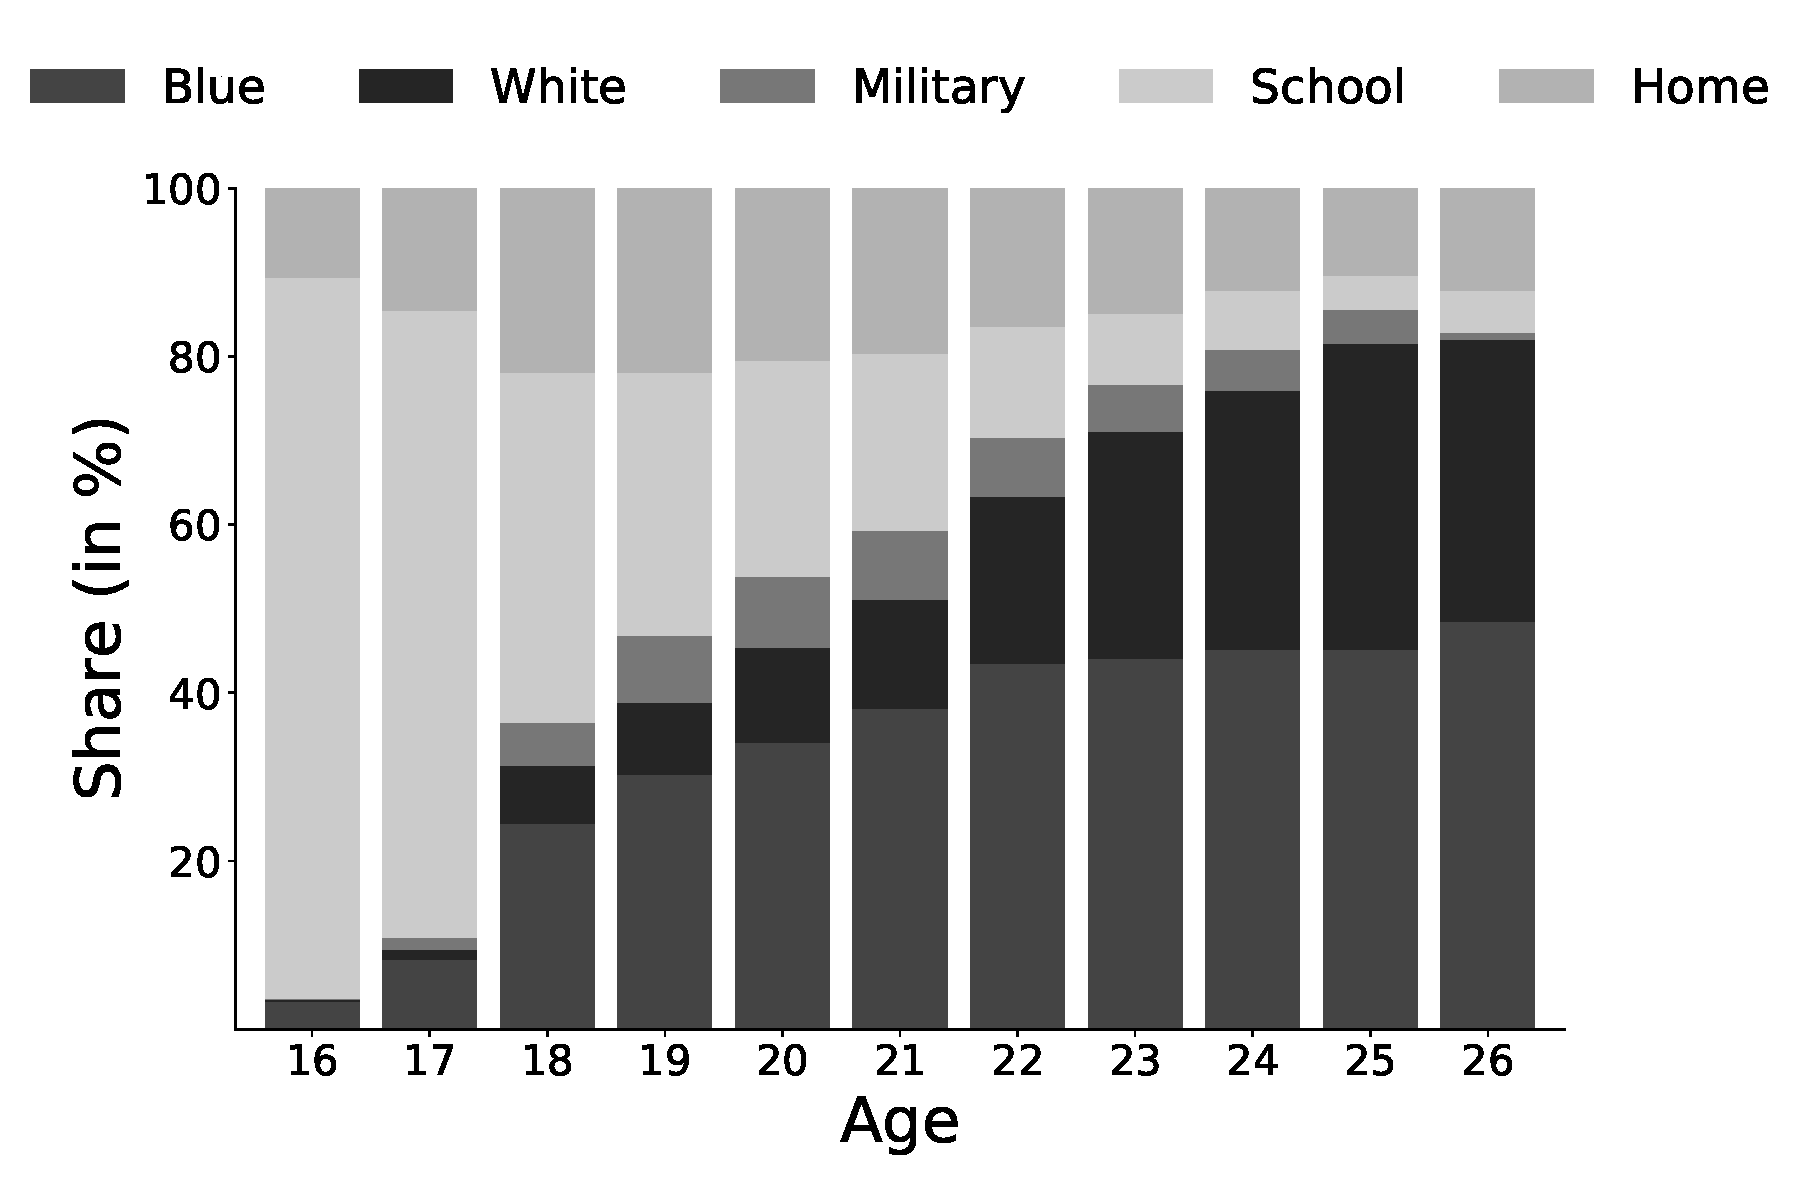
\includegraphics{fig-data-choice-all-bw}}}\hspace{0.3cm}
\subfloat[Average wage]{\scalebox{0.25}{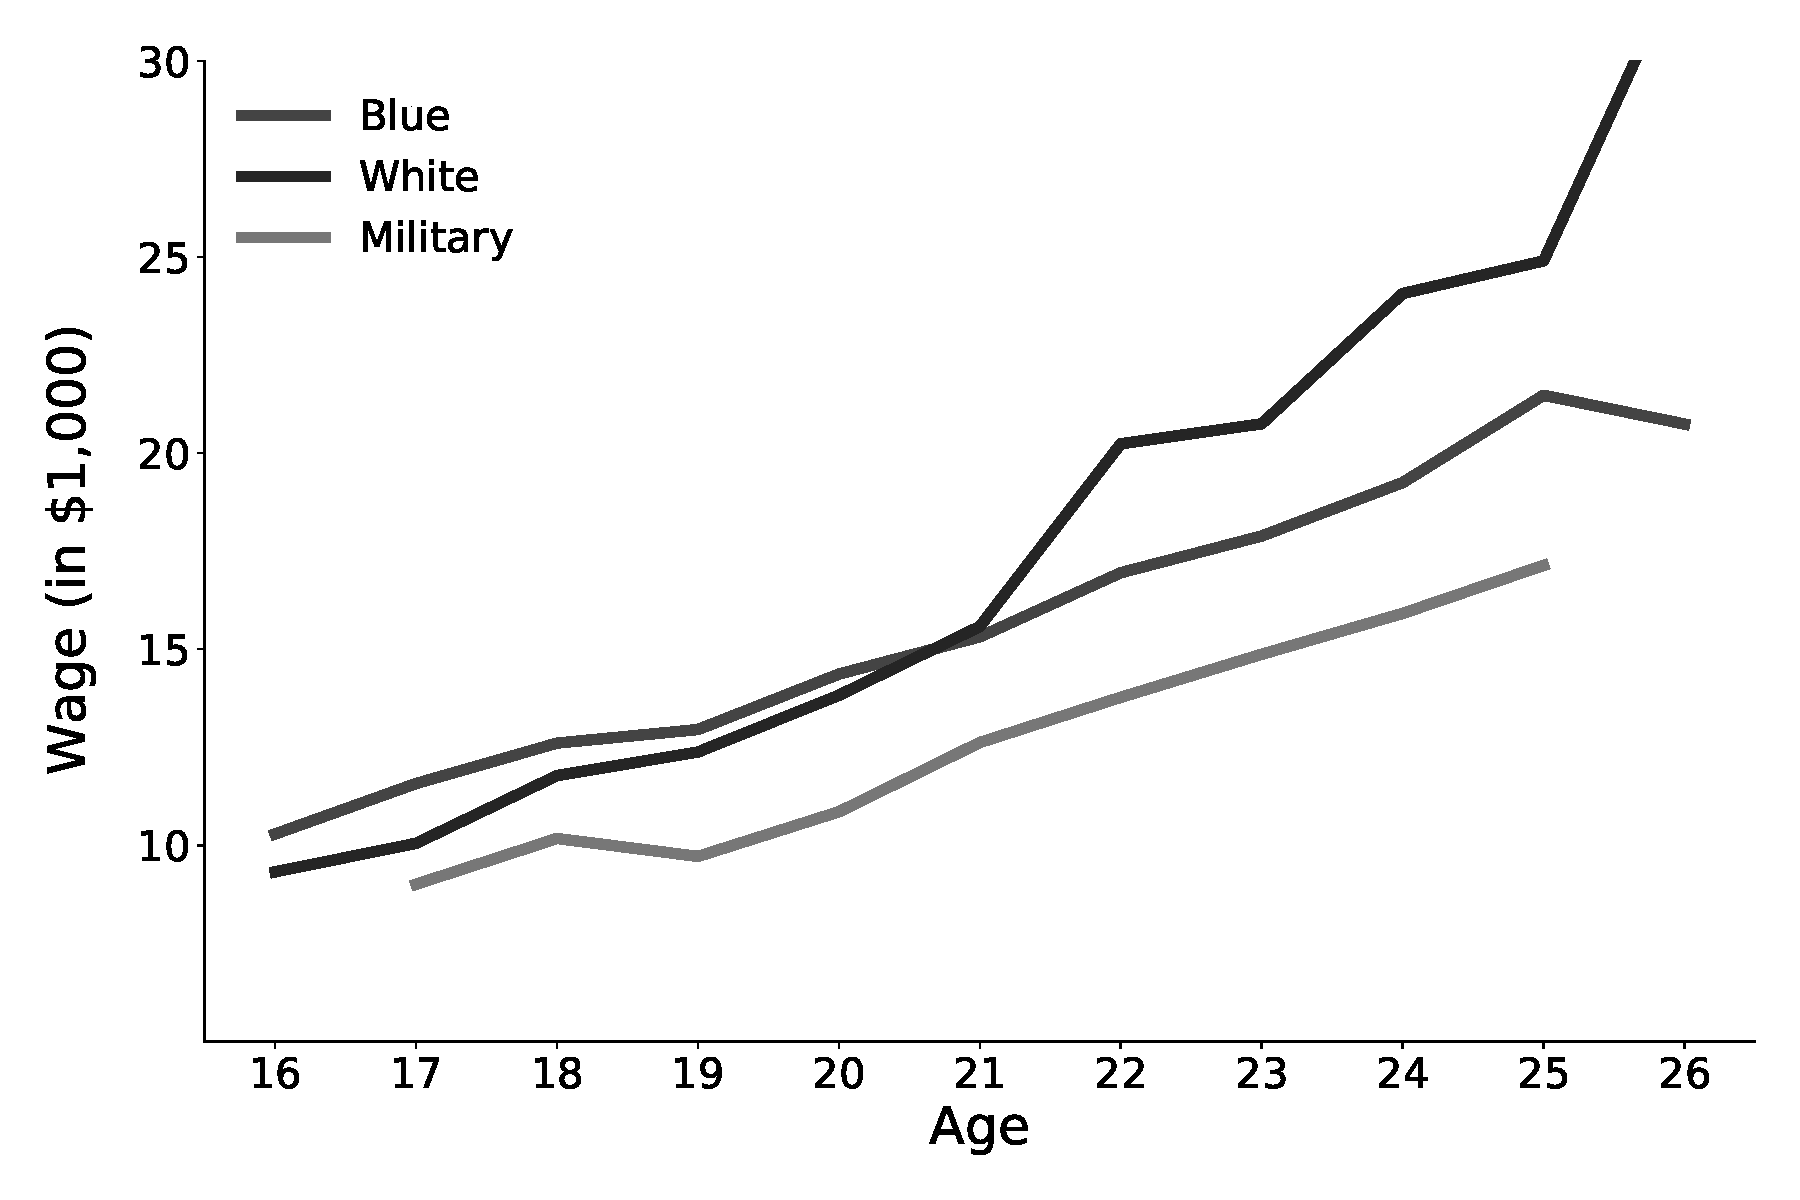
\includegraphics{fig-data-wage-occupations-bw}}}
\begin{center}
\begin{minipage}[t]{0.75\columnwidth}
\item \scriptsize{\textbf{Notes:} The wage is a full-time equivalent deflated by the gross national product deflator, with 1987 as the base year. We do not report the wage if less than ten observations are available.}
\end{minipage}
\end{center}
\end{figure}\FloatBarrier
%
\noindent Overall, average wages start at about \$10,000 at age 16 but increase considerably up to about \$25,000 at age 26. While wages in the blue-collar occupation are initially highest with about \$10,286, wages in the white-collar occupation and military start around \$9,000. However, wages in the white-collar occupation increase steeper over time and overtake blue-collar wages around age 21. At the end of the observation period, wages in the white-collar occupation are about 50\% higher than blue-collar wages with \$32,756 as opposed to only \$20,739. Military wages remain lowest throughout.\\

\noindent We fit the model to the empirical data using maximum likelihood calibration. Figure \ref{Model fit} shows the overall agreement between the empirical data and a dataset simulated using the calibrated parameters within the support of the data. On the left, we show the choice probability of working in a blue-collar occupation, while we plot the average wage across all occupations on the right.
%
\begin{figure}[h!]\centering
\caption{Model fit}\label{Model fit}
\subfloat[Blue-collar]{\scalebox{0.25}{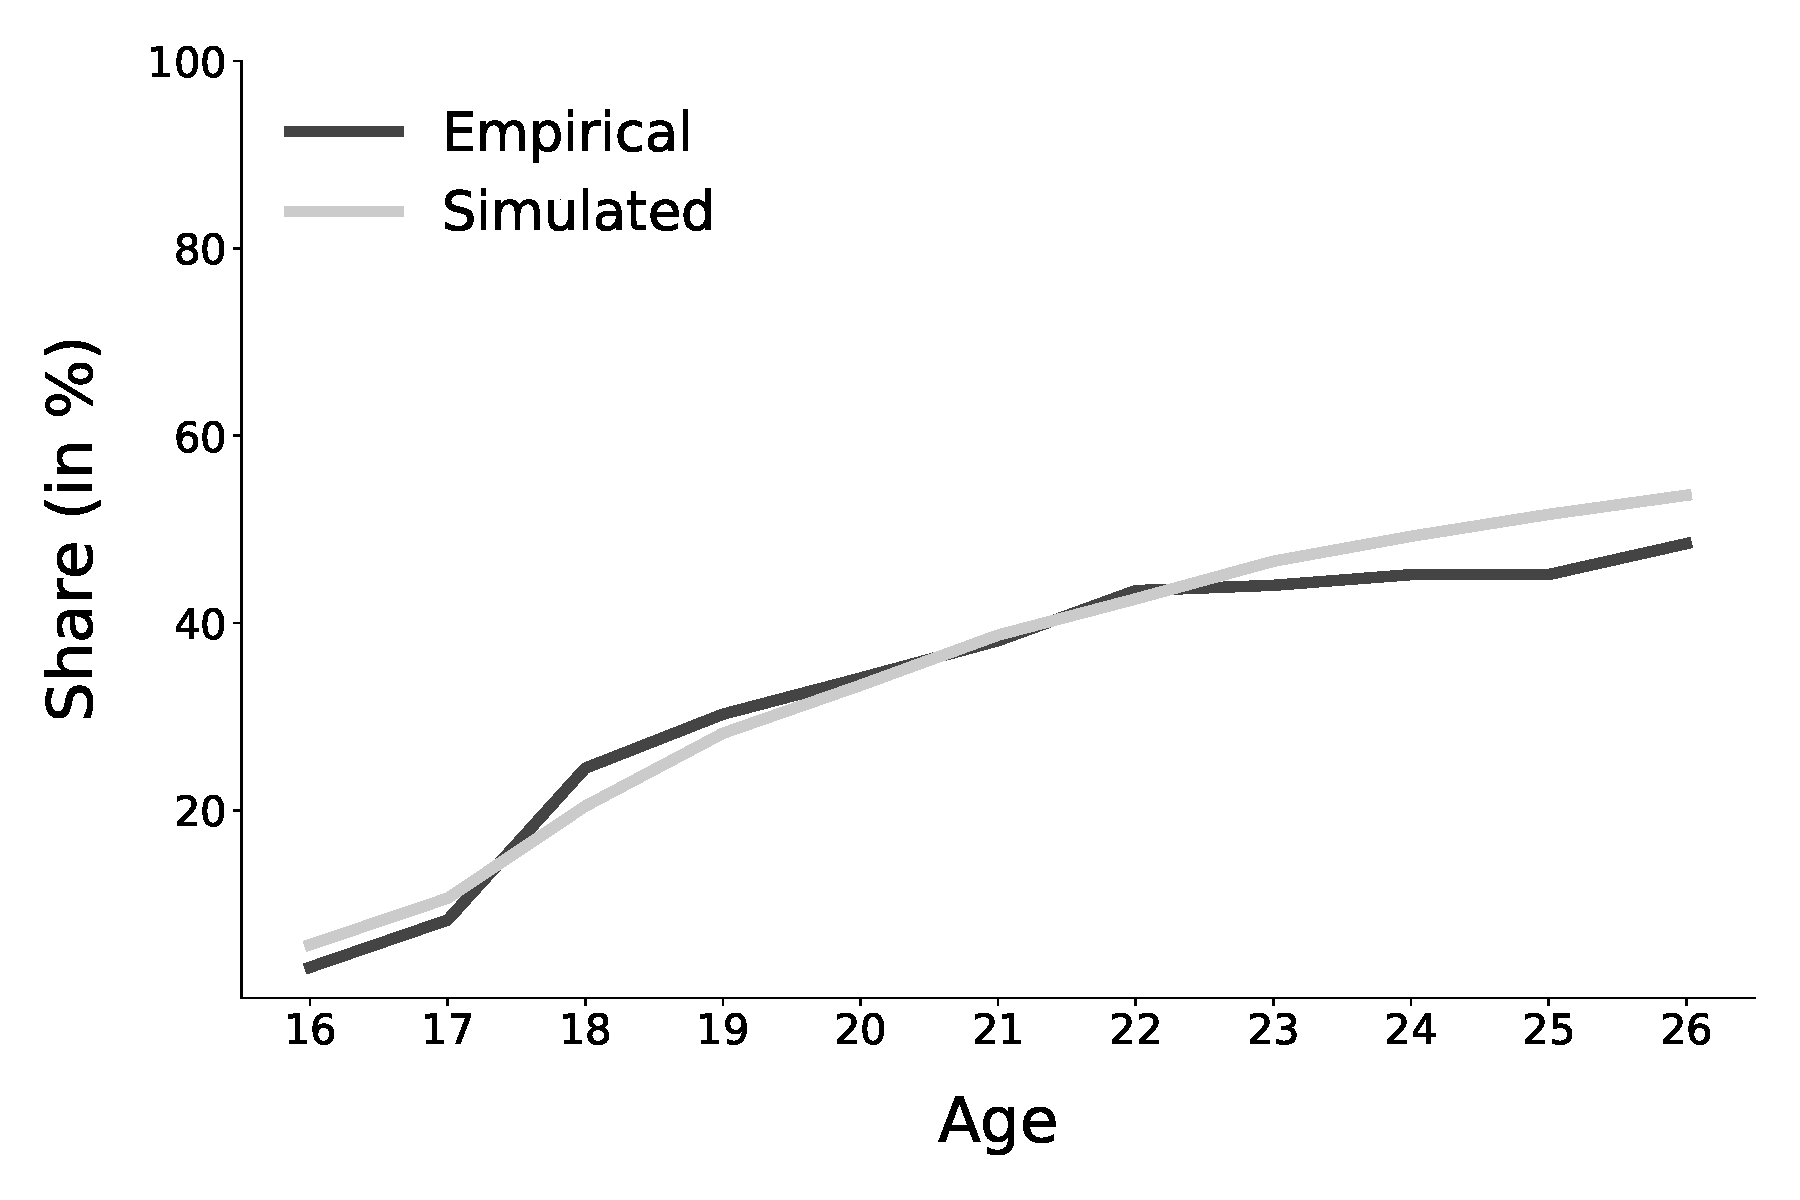
\includegraphics{fig-model-fit-choice-blue-bw}}}\hspace{0.3cm}
\subfloat[Average wage]{\scalebox{0.25}{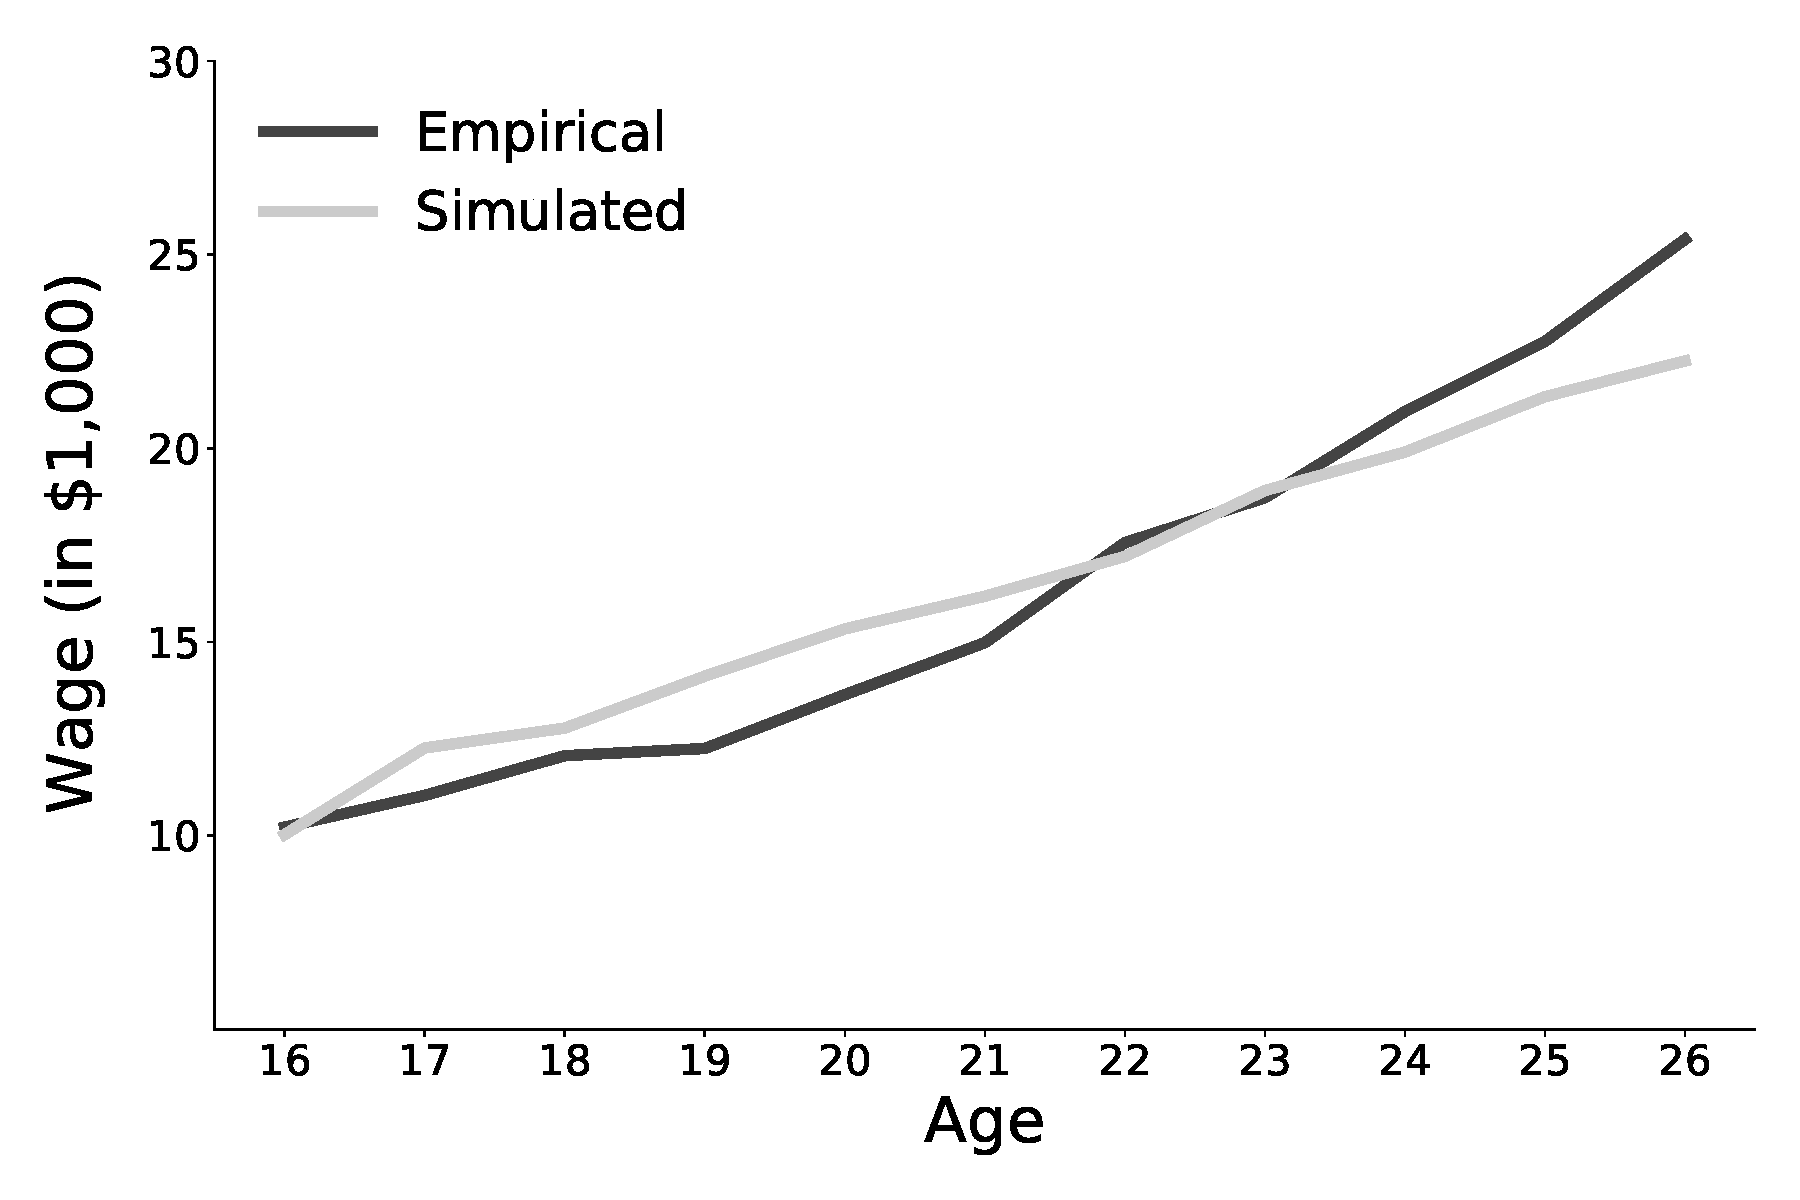
\includegraphics{fig-model-fit-wage-all-bw}}}
\begin{center}
\begin{minipage}[t]{0.60\columnwidth}
\item \scriptsize{\textbf{Notes:} We simulate a sample of 1,000 individuals using the calibrated model.}
\end{minipage}\end{center}
\end{figure}\FloatBarrier
%
\noindent Overall, the values of the calibrated parameters of the model are in broad agreement with the relevant literature. For example, individuals discount future utilities by $6\%$ per year, and wages increase by about $7\%$ with each additional year of schooling.
%-------------------------------------------------------------------------------
\subsection{Economic insights}
%-------------------------------------------------------------------------------
Figure \ref{Economic mechanism and policy forecast} illustrates the ability of the model to quantify the impact of economic mechanisms and to forecast the effect of public policies. On the left, we vary the discount factor capturing time preferences between $0.91$ and $0.95$ while we introduce a tuition subsidy of up to $\$4,000$ on the right. In both cases, we are interested in the changes to average final schooling.

\begin{figure}[h!]\centering
\caption{Economic mechanism and policy forecast}\label{Economic mechanism and policy forecast}
\subfloat[Time preference]{\scalebox{0.25}{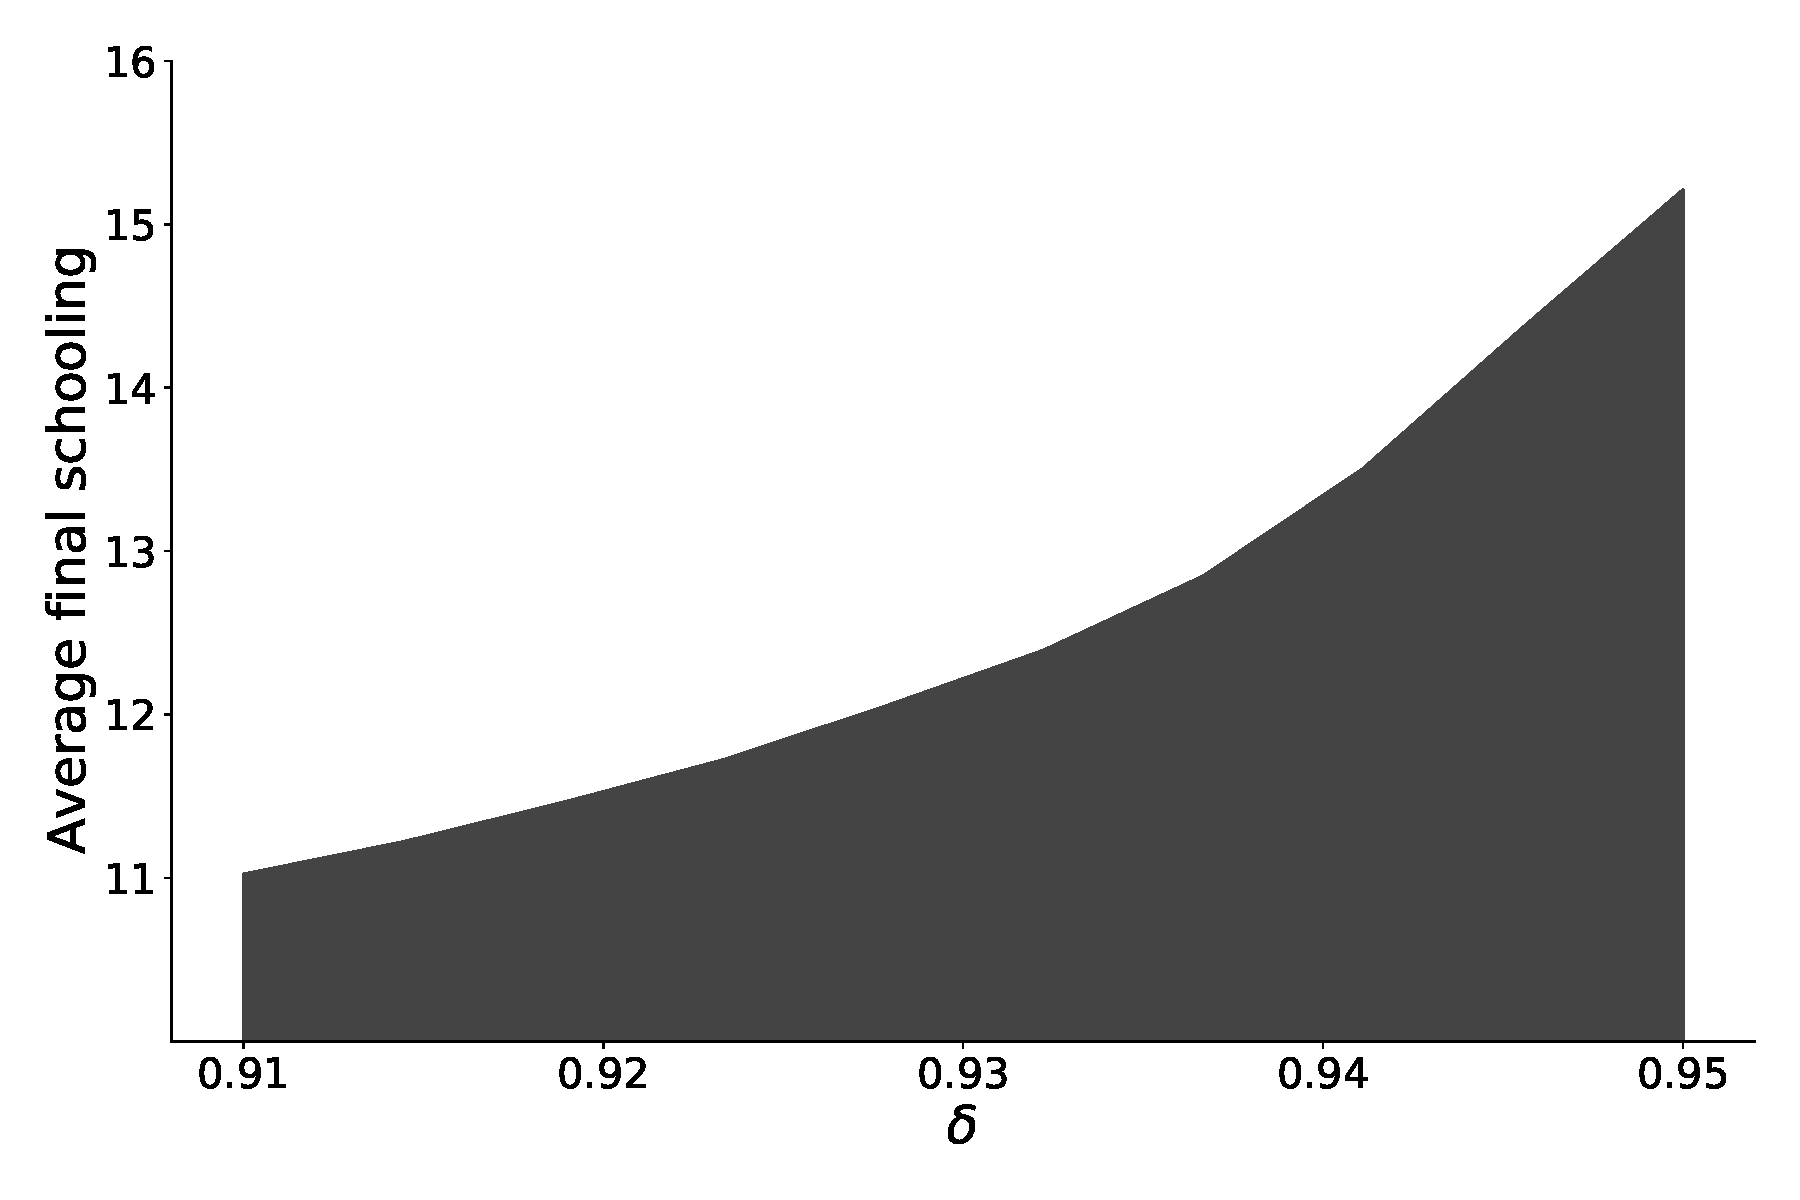
\includegraphics{fig-economic-mechanism-bw}}}\hspace{0.3cm}
\subfloat[Tuition subsidy]{\scalebox{0.25}{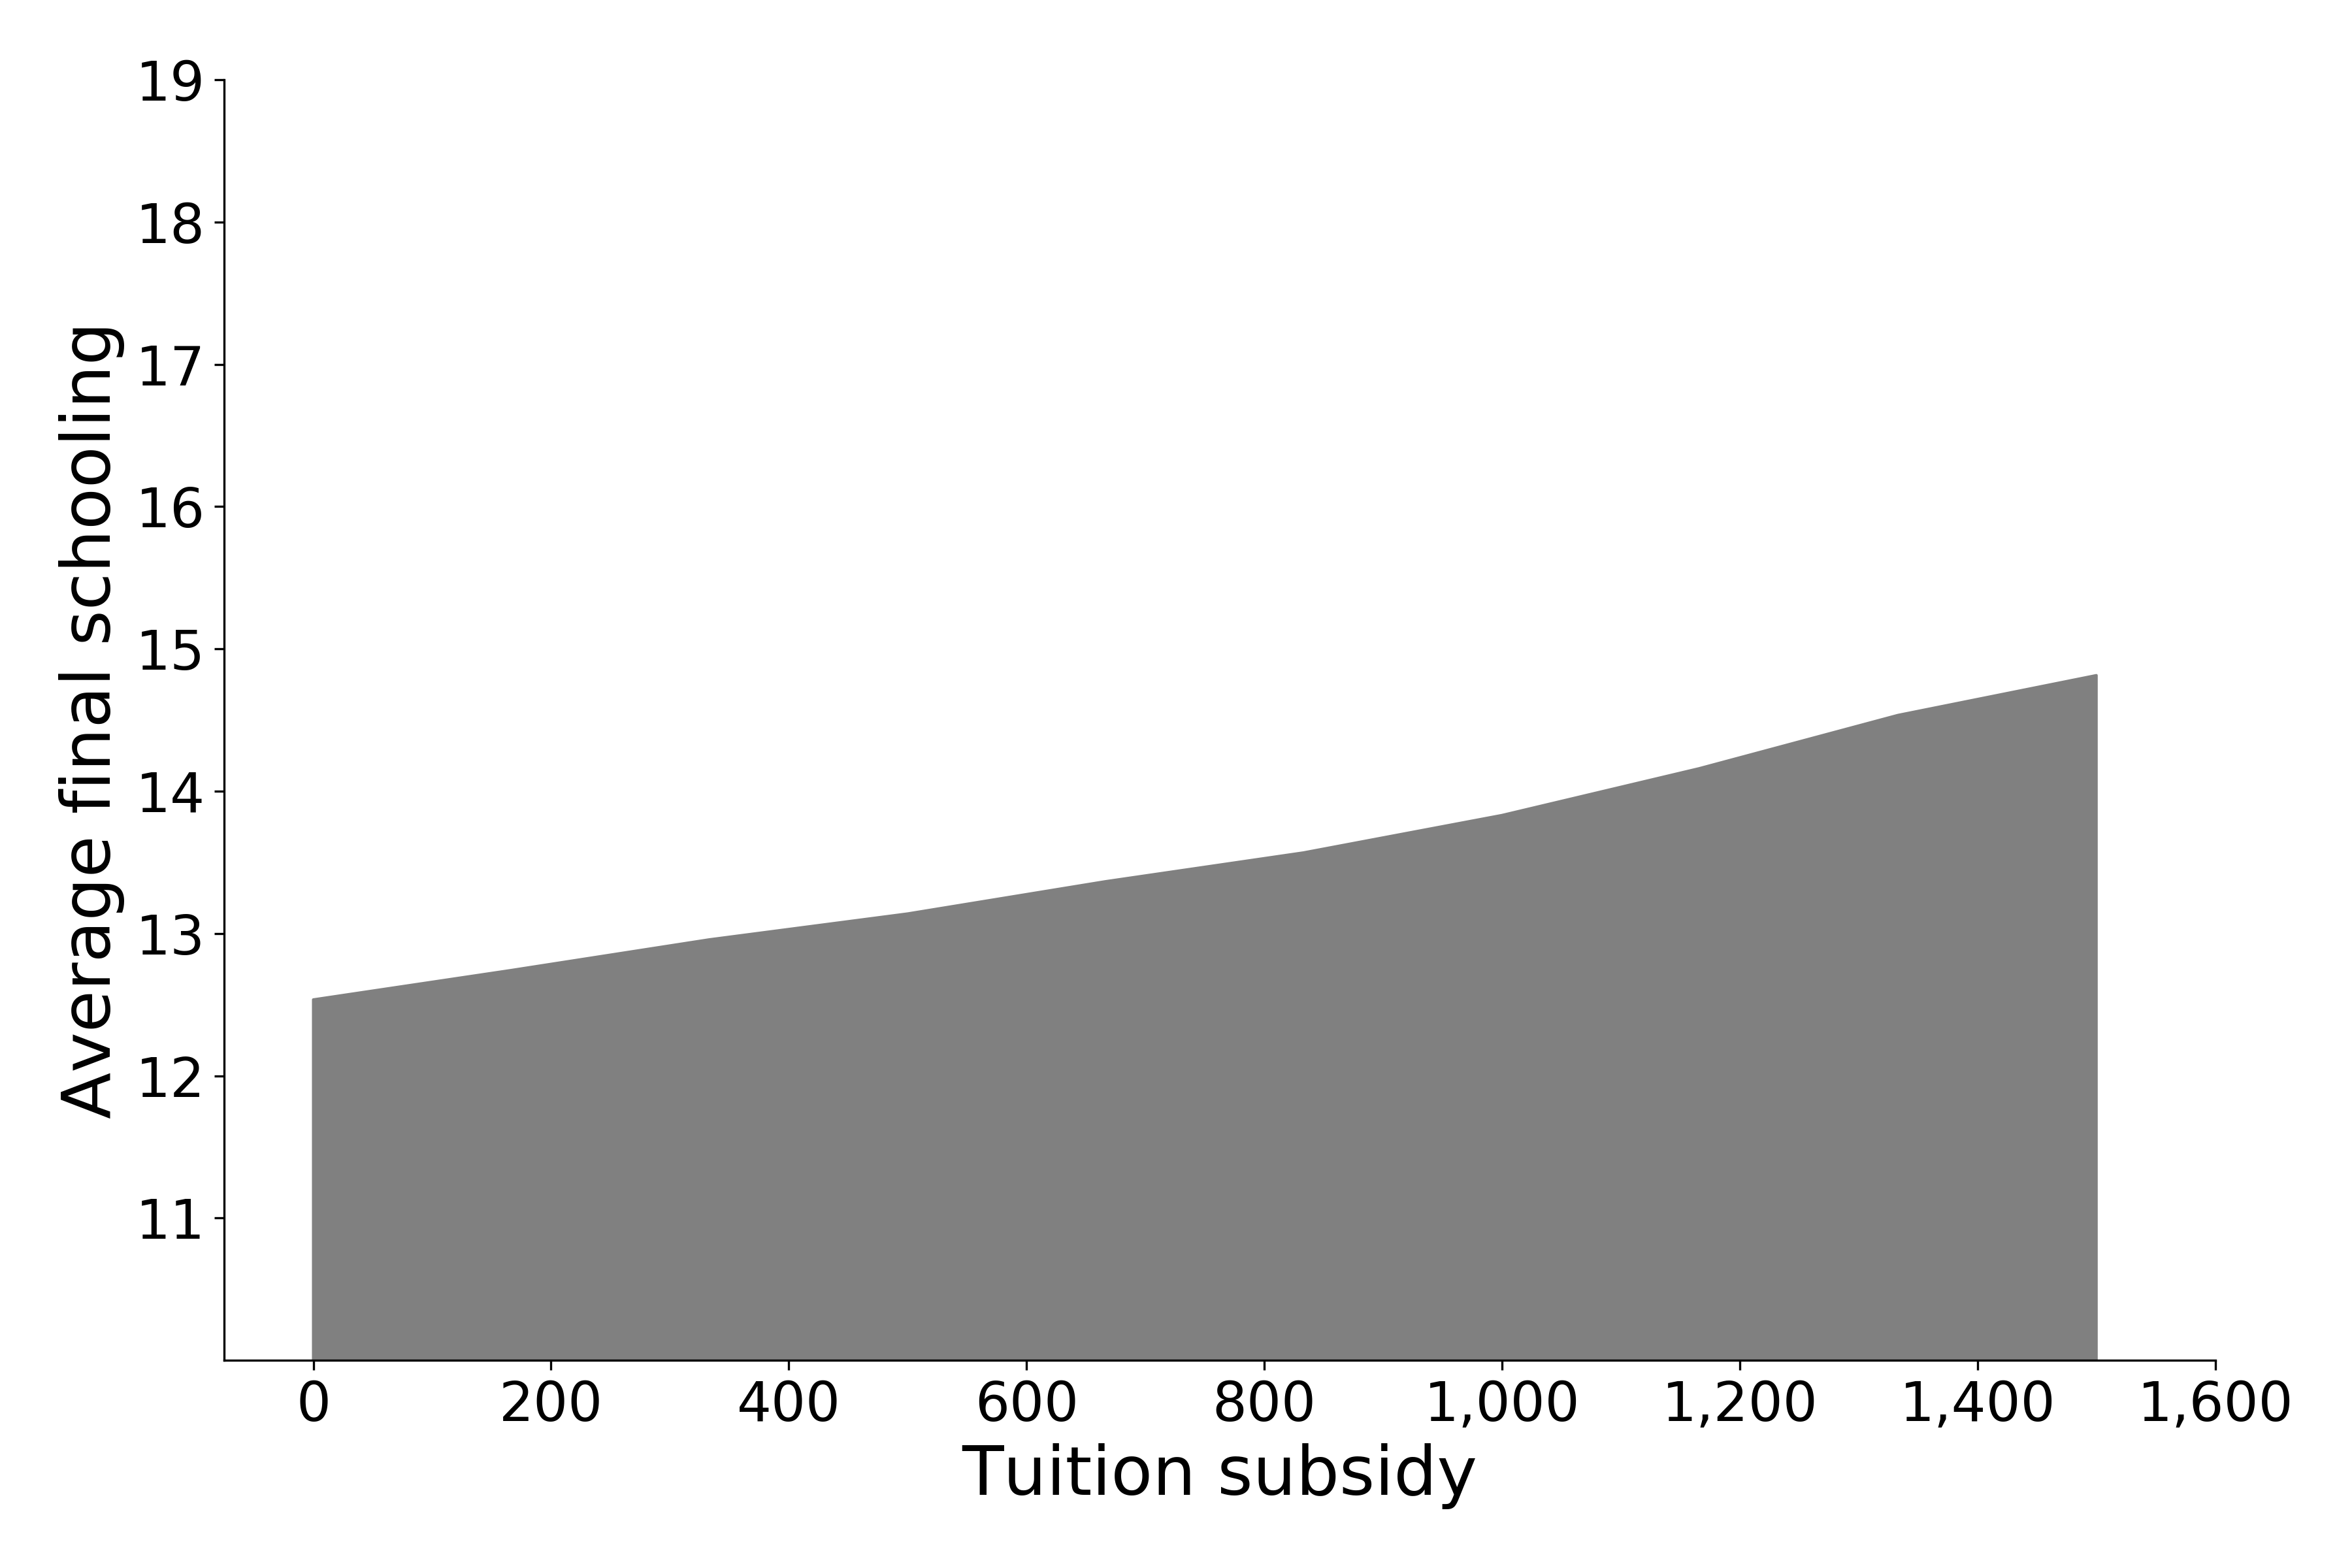
\includegraphics{fig-policy-forecast-bw}}}
\begin{center}
\begin{minipage}[t]{0.60\columnwidth}
\item \scriptsize{\textbf{Notes:} We simulate a sample of 1,000 individuals using the calibrated model.}
\end{minipage}
\end{center}
\end{figure}\FloatBarrier

\noindent Increases in the discount factor and the tuition subsidy both result in higher average final schooling. However, they do so for very different reasons. While individuals emphasize the future benefits of their schooling investment in the former, they react to a reduction of its immediate cost in the latter.
